% Copyright 2006 by Till Tantau
%
% This file may be distributed and/or modified
%
% 1. under the LaTeX Project Public License and/or
% 2. under the GNU Free Documentation License.
%
% See the file doc/generic/pgf/licenses/LICENSE for more details.


\section{Matrices}

\label{section-base-matrices}

\subsection{Overview}

Matrices are a mechanism for aligning several so-called cell pictures 
horizontally and vertically. The resulting alignment is placed in a
normal node and the command for creating matrices, |\pgfmatrix|, takes
options very similar to the |\pgfnode| command.

In the following, the basic idea behind the alignment mechanism is
explained first. Then the command |\pgfmatrix| is explained. At the
end of the section additional ways of modifying the width of columns
and rows is discussed.


\subsection{Cell Pictures and Their Alignment}

A matrix consists of rows of \emph{cells}. Cells are separated using
the special command |\pgfmatrixnextcell|, rows are ended using the
command |\\|. Each cell contains a \emph{cell picture}, although cell
pictures are not complete pictures as they lack layers. However, each
cell picture has its own bouding box like a normal picture does. These
bounding boxes are important for the alignment as explained
in the following.

Each cell picture will have an origin somewhere in the picture (or
even outside the picture). The position of these origins is important
for the alignment: On each row the origins will be on the same
horizontal line and for each column the origins will also be on the
same vertical line. These two requirements mean that the cell pictures
may need to be shifted around so that the origins wind up on the same
lines. The top of a row is given by the top of the cell picture whose
bounding box's maximum $y$-position is largest. Similarly, the bottom
of a row is given by the bottom of the cell picture whose bounding
box's minimum $y$-position is the most negative. Similarly, the left
end of a row is given by the left end of the cell whose bounding box's
$x$-position is the most negative; and similarly for the right end of
a row.

\begin{codeexample}[]
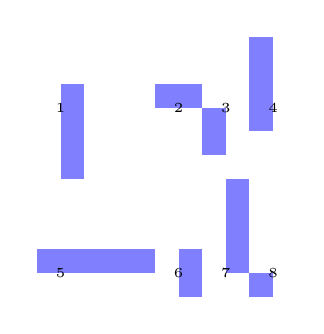
\begin{tikzpicture}[x=3mm,y=3mm,fill=blue!50]
  \def\atorig#1{\node[black] at (0,0) {\tiny #1};}

  \pgfmatrix{rectangle}{center}{mymatrix}
    {\pgfusepath{}}{\pgfpointorigin}{}
    {
      \fill (0,-3)  rectangle (1,1);\atorig1 \pgfmatrixnextcell
      \fill (-1,0)  rectangle (1,1);\atorig2 \pgfmatrixnextcell
      \fill (-1,-2) rectangle (0,0);\atorig3 \pgfmatrixnextcell
      \fill (-1,-1) rectangle (0,3);\atorig4 \\
      \fill (-1,0)  rectangle (4,1);\atorig5 \pgfmatrixnextcell
      \fill (0,-1)  rectangle (1,1);\atorig6 \pgfmatrixnextcell
      \fill (0,0)   rectangle (1,4);\atorig7 \pgfmatrixnextcell
      \fill (-1,-1) rectangle (0,0);\atorig8 \\
    }
\end{tikzpicture}
\end{codeexample}


\subsection{The Matrix Command}

All matrices are typeset using the following command:

\begin{command}{\pgfmatrix\marg{shape}\marg{anchor}\marg{name}%
    \marg{usage}\marg{shift}\marg{pre-code}\marg{matrix cells}}
  ...
\end{command}


%%% Local Variables: 
%%% mode: latex
%%% TeX-master: "pgfmanual"
%%% End: 
